\clearpage
\section{Bartosz Sendor}

\subsection{Matematyka}
Oto przykład nieprzyjemnego zadania z analizy:

        \[\lim_{n\to\infty} \frac{1}{1+n^2}+\frac{2}{2+n^2}+\dots+\frac{n}{n+n^2}=?\]
Rozwiązanie
        \[ \frac{c}{n+n^2} \leq \frac{c}{c+n^2} \leq \frac{c}{1+n^2} \]
        dla \(c \in N\), więc
\begin{align*}
    & \frac{1}{n+n^2}+\frac{2}{n+n^2}+\dots+\frac{n}{n+n^2} \leq \\
    \leq & \frac{1}{1+n^2}+\frac{2}{2+n^2}+\dots+\frac{n}{n+n^2} \leq \\
    \leq & \frac{1}{1+n^2}+\frac{2}{1+n^2}+\dots+\frac{n}{1+n^2}\\\\
\end{align*}
Z twierdzenia o trzech ciągach
    \[\lim_{n\to\infty} \frac{\frac{1}{2}n(n+1)}{n+n^2} \leq
    \lim_{n\to\infty} \frac{1}{1+n^2}+\frac{2}{2+n^2}+\dots+\frac{n}{n+n^2} \leq
    \lim_{n\to\infty} \frac{\frac{1}{2}n(n+1)}{1+n^2} \]
    \[\frac{1}{2} \leq
    \lim_{n\to\infty} \frac{1}{1+n^2}+\frac{2}{2+n^2}+\dots+\frac{n}{n+n^2} \leq
    \frac{1}{2}\]
    \[\lim_{n\to\infty} \frac{1}{1+n^2}+\frac{2}{2+n^2}+\dots+\frac{n}{n+n^2}=\frac{1}{2}\]




\subsection{Zdjęcie}
\label{fig: scierwojad}

\begin{figure}[h]
    \centering
    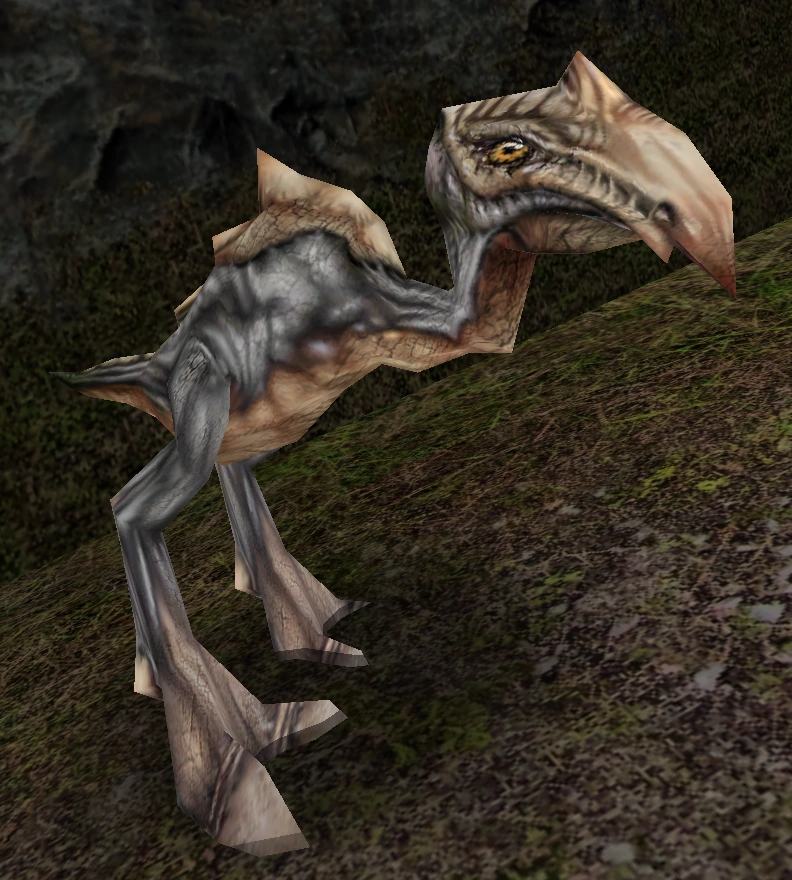
\includegraphics[height = 200pt]{pictures/BartekSendor.png}
    \caption{Ścierwojady, tak nazywamy te wielkie ptaszyska, należy atakować jeden po drugim}
\end{figure}

\newpage

\subsection{Tabela: Składniki na potrawkę z chrząszcza a la Snaf}
\label{tab: ściganie}

\begin{table}[h!]
\centering
\begin{tabular}{|c|c|c|c|c|}
\hline
\textbf{Składniki} & dla 1 osoby & dla 2 osób & dla 3 osób& dla 4 osób\\ \hline
Ciemne grzyby           & 5     &10     &15     &20    \\ \hline
Mięso z chrząszcza      & 3     &6      &9      &12    \\ \hline
\end{tabular}
\end{table}


\subsection{Lista Iana (numerowana)}

\begin{enumerate}
    \item 20 bochenków chleba
    \item 25-30 jabłek
    \item 10 kawałków sera
    \item 1 chochla
    \item 1 szcztoka
    \item 5 kilofów + 3 młotki
\end{enumerate}

\subsection{Lista Iana (nienumerowana)}

\begin{itemize}
    \item 20 bochenków chleba
    \item 25-30 jabłek
    \item 10 kawałków sera
    \item 1 chochla
    \item 1 szcztoka
    \item 5 kilofów + 3 młotki
\end{itemize}

\subsection{List do arcymistrza magów kręgu ognia}

\textbf{Czcigodny Mistrzu},\\

Twój ostatni list napełnił nas wielkim smutkiem. Po rozważeniu sprawy, niniejszym przedstawiamy nasze stanowisko w tej sprawie: \underline{Bractwo stało się} \underline{poważnym zagrożeniem dla całej kolonii}. Jego działania narażają na niebezpieczeństwo nasze delikatne pertraktacje handlowe z \emph{Jego Wysokością}, a tym samym - przyszłe losy całego królestwa. Dlatego zalecamy wysłanie do obozu na bagnie grupy zwiadowców, którzy ustalą z jakiegoż piekielnego źródła członkowie Bractwa czerpią swą moc. Posiadając te informacje moglibyśmy połączyć nasze wysiłki w celu rychłego zażegnania niebezpieczeństwa. Nasi Bracia przeszukują obecnie prastare księgi w poszukiwaniu choćby najmniejszego znaku, który mógłby naprowadzić nas na właściwy trop. O wynikach tych poszukiwań poinformujemy zwykłą drogą.\\

\emph{\textbf{\large Niech Innos ma w opiece nas wszystkich. \normalsize}}